\section{Análisis del proceso actual}
A continuación se describe el proceso para reportar incidentes por parte de los ciudadanos a través del servicio
de emergencia Ecu 911. Este proceso se basa en la información obtenida de la entrevista realizada al teniente
coronel de estado mayor Christian Iván Quintana Guerra, En la Figura 1 se detalla el siguiente proceso, donde:

\begin{enumerate}
    \item El usuario llama al número de emergencia del ECU 911.
    \item El operador recibe la llamada y solicita la información necesaria al usuario.
    \item En base al tipo de incidente, el operador asigna la emergencia a la entidad correspondiente.
    \item La entidad correspondiente recibe la emergencia y envía una unidad al lugar del incidente.
    \item La unidad llega al lugar del incidente, donde:
          \begin{enumerate}
              \item La unidad verifica la información con la que cuenta:
                    \begin{enumerate}
                        \item Si cuenta con la información necesaria, la emergencia es atendida.
                        \item Si no cuenta con la información necesaria, se solicita a la víctima o testigo la información faltante.
                    \end{enumerate}
          \end{enumerate}
    \item Se reporta el incidente la atención de la emergencia y la información es almacenada en una matriz de excel.
\end{enumerate}

\begin{figure}[H]
    \centering
    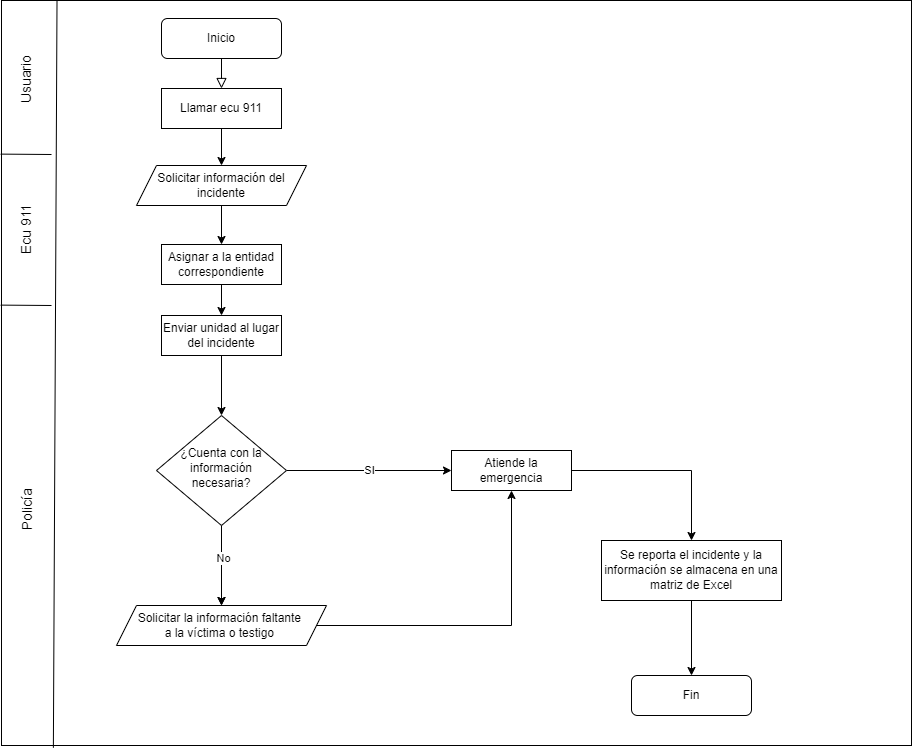
\includegraphics[width=0.8\textwidth]{chapters/III-resultados-y-discusion/resources/images/proceso-actual.png}
    \caption{Proceso actual de reporte de incidentes al ECU 911.}
    \label{fig:proceso-actual}
\end{figure}